% -*- mode: fundamental -*-

% ****************************************************************

\chapter{RISC-V interpreters: the Design Space  \\
from Software Functional Simulators to High-Performance Hardware}

\markboth{Ch \arabic{chapter}: Design Space}{\copyrightnotice}

\setcounter{page}{1}
% \renewcommand{\thepage}{\arabic{page}}
\renewcommand{\thepage}{\arabic{chapter}-\arabic{page}}

\label{ch_RISCV_Design_Space}

% ****************************************************************

Any artefact/engine that executes the instructions of any ISA is an
\emph{interpreter} for that ISA. The classical meaning of an
interpreter is an algorithm (program) that examines/traverses a data
structure that is itself the represention of a target program, and
performs actions accordingly.  In our case, the target program is a
RISC-V binary and the data structure is an array or RISC-V
instructions.  The algorithm examines RISC-V instructions in the
array, conceptually one-instruction-at-a-time, and performs the
instruction's actions.

Any algorithm can be implemented in software or in hardware.  Further,
the boundary is fluid: parts of the algorithm can be implemented in
software, cooperating with other parts that are implemented in
hardware (``accelerators'').  The choice between software and hardware
implementation is pragmatic (speed, power, cost, cost of debugging and
modification, cost of redesign, {\etc}); functionally there is no
theoretical difference.

When we implement an ISA interpreter in software, we call it a
``simulator''.  When we implement it in hardware, we call it a
hardware implementation.  Both software simulators and hardware
implementations can vary widely in microarchitecture.  Some design
options are:

\begin{itemize}

  \item Sequential or pipelined?  One full instruction at-a-time, or
    multiple instructions flowing through a pipe, each at a more
    advanced step in its execution than the one behind it.

  \item Predictive (in pipelined implementations)?  {\Eg} predict what
    instructions to fetch while a BRANCH/JUMP flows through the pipe
    before we know the actual next-instruction determined the
    BRANCH/JUMP.

  \item Superscalar/VLIW? Fetch and execute more than one instruction
    in parallel, taking care to preserve sequential ISA semantics.

  \item Out-of-order? Execute each instruction as soon as its input
    data is available, without waiting for prior instructions which
    may still be waiting for their inputs.

\end{itemize}

For the same microarchitecture, a software simulator is typically
\emph{much slower} than a hardware implementation.  This is because it
involves (at least) two layers of simulation.  The software simulator
is itself a program that is being interpreted, perhaps directly in
hardware.  That program (the simulator), in turn, is interpreting the
target ISA.  The two interpreters need not and may not be for the same
ISA.  For example, if we run a RISC-V software simulator on a modern
server, the lower level may be an x86 or ARM interpreter ({\ie} the
CPU in in the server).  A software simulator written in Python or Java
involves three layers of ISAs, {\eg} hardware x86/ARM interpreting
x86/ARM instructions representing a program to interpret bytecode
(second level ISA), which, in turn represents an interpreter for
RISC-V programs.  Every additional layer of interpretation can slow
down overall performance by possibly orders of magnitude.

Paradoxically, adding any of the microarchitectural details mentioned
in the list above will normally slow down a software simulator but
speed up a hardware implementation.  This is because those
microarchitetural details expose more \emph{parallelism} and
\emph{concurrency} in the interpretation algorithm.  Hardware
implementations actually execute these parallel actions in parallel,
whereas a software simulator (written, say, in C/C++) may execute them
sequentially ({\ie} \emph{modeling} parallelism but in fact being
sequential).  Of course, the extra hardware speed is not free: it
needs more hardware and more complexity in the design (cost, power
consumption).

% ****************************************************************

\section{The RISC-V designs in this book}

In this book we will focus on two simple hardware implementations,
Both designs are coded in BSV, a free, open-source, modern, High-Level
Hardware Design Language (HLHDL).  BSV code can be compiled into
Verilog, which can then be run on any Verilog simulator, or can be
further processed by FPGA tools to run on FPGAs, or by ASIC tools for
ASIC implemenetations.  For more discussion of our choice of BSV,
please see Appendix~\ref{apx_Why_BSV}.

Our first hardware RISC-V implementation---``Drum''---will be a
simple one-full-instruction-at-a-time interpereter, almost a direct
transliteration into BSV code of the generic ISA execution algorithm
to be described next in Section~\ref{Sec_ISA_Exec_Algorithm}.  It does
not implement any interesting microarchitectural feature, not even
pipelining, which is the most basic microarchitectural feature of most
CPU implementations.  Lacking microarchitectural features, in fact the
BSV code will look very similar to what you might write in C/C++ for a
purely functional RISC-V simulator.  Being written in BSV, however, we
can compile and run it on actual hardware (FPGAs, ASICs).

Drum will not be fast compared to other hardware CPUs, because of lack
of microarchitectural features, but we should still be able to run it
at several 100 MHz on an FPGA, which will make it faster than many
software functional simulators.  It will be small (silicon area, and
therefore low power as well).  Drum is covered from
Chapter~\ref{ch_core_functions} through Chapter~\ref{ch_Drum_code}.

Our second implementation---``Fife''---adds pipelining.  Pipelining
introduces new complications because of potential interaction between
instructions that are at different stages in the pipe.  We can focus
on these new complications because all the functional aspects of
RISC-V ISA execution have already been addressed in Drum.  In fact, we
will reuse the functional code from Drum without change.  Fife is
covered in Chapter~\ref{ch_Fife_Principles} through
Chapter~\ref{ch_Fife_code}.

For both Drum and Fife, we will focus initially on only the RV32I
option of the RISC-V ISA.  Please refer to the specification document
``The RISC-V Instruction Set Manual Volume I: Unprivileged
ISA''~\cite{RISCV_Unpriv_2019_12_13}.  In particular, look at Chapter
24 ``RV32/64G Instruction Set Listings'', and the first table therein,
entitled ``RV32I Base Instruction Set'', showing forty instructions.
These instructions are describe in more detail in the same document in
Chapter 2 ``RV32I Base Integer Instruction Set, Version 2.1''.

We will extend this with just enough functionality to be able to
recover from illegal instructions ({\ie} an instruction outside the
set of forty RV32I instructions) and to handle interrupts.  This
minimal functionality will be taken from the specficitation document
``The RISC-V Instruction Set Manual Volume II: Privileged
Architecture''\cite{RISCV_Priv_2021_12_03}.

Beyond this book, we extend Drum and Fife to handle RV64I and more
Unprivileged ISA options---M: integer multiply/divide, A: atomics, FD:
single-and double-precision floating point, and C: compressed. We also
handle more privileged ISA options---Privilege levels (M: Machine, S:
Supervisor and U:User; full complement of Control and Status Registers
(CSRs); Virtual Memory).  With these extensions, Drum and Fife
will be able to a full-feature Operating System (OS), such as Linux.

% ****************************************************************

\section{Abstract algorithm for interpreting an ISA}

\label{Sec_ISA_Exec_Algorithm}

\index{RISC-V!Architectural state}

From our previous study of the RISC-V ISA, we know that the basic
integer ``architectural state'' of a RISC-V CPU is very simple:

\begin{itemize}

\item A ``program counter'' (PC) indicating the address in memory of
the next instruction to be executed.

\item A ``register file'' consisting of 32 general purpose registers
(GPRs), each containing data.

\end{itemize}

The PC and each register are either 32-bits wide (in the RV32 option
of RISC-V) or 64-bits wide (in the RV64 option).  For simplicity,
we'll focus on RV32 here, but everything we discuss also applies to
RV64.

Interpreting a program involves the repetition of a few simple
steps,\footnote{We prefer the word ``step'' here instead of ``stage'',
which we will reserve to refer to stages in a hardware pipeline such
as Fife.}  illustrated in
Figure~\ref{Fig_Instr_Exec}:
\begin{figure}[htbp]
  \centerline{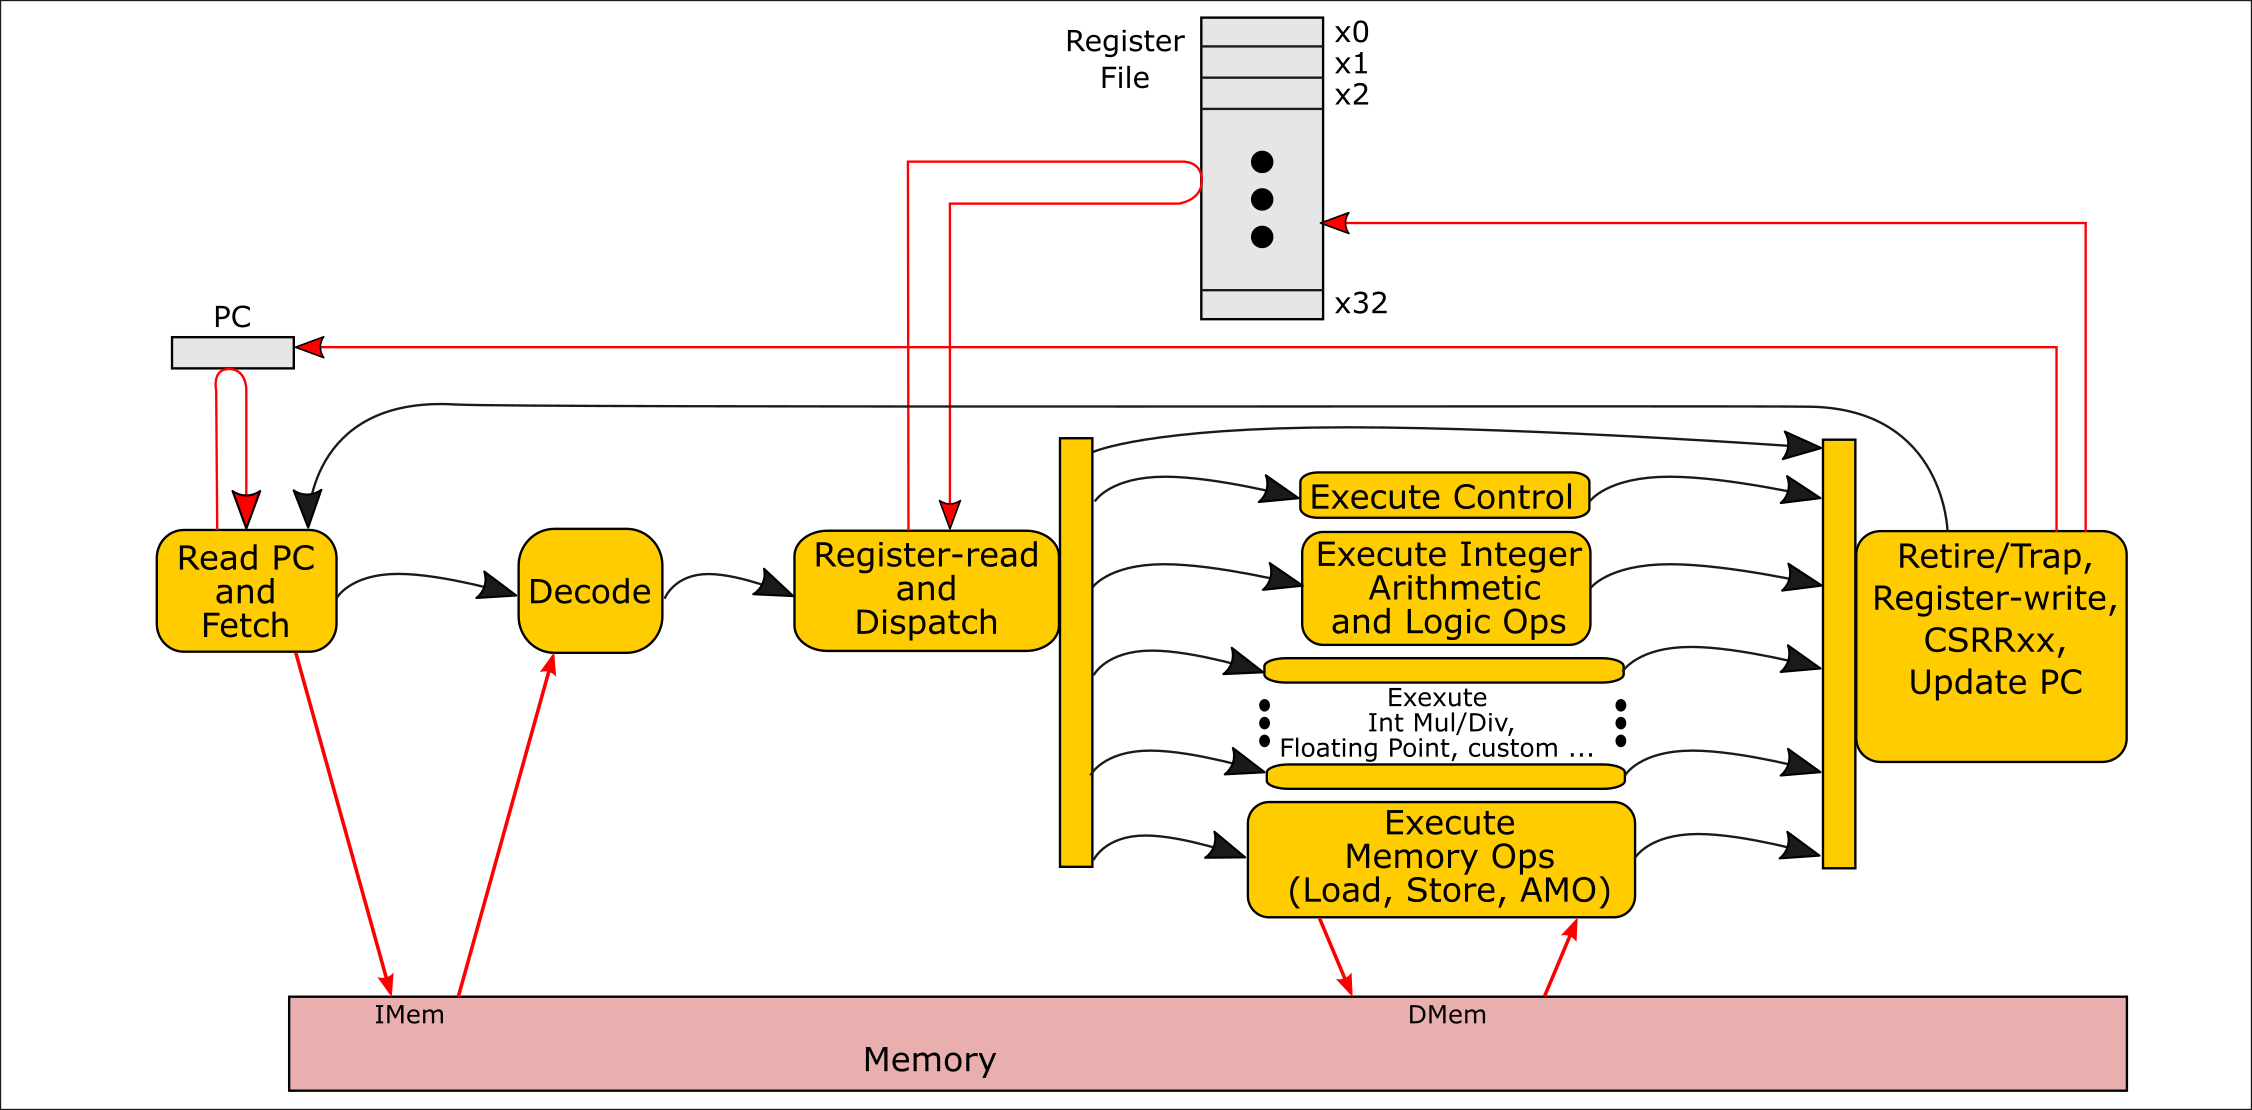
\includegraphics[width=6in,angle=0]{Figures/Fig_Instr_Exec}}
  \caption{\label{Fig_Instr_Exec}Simple interpretation of RISC-V instructions}
\end{figure}
\begin{itemize}

\item The ``Fetch'' step reads the current value of the PC and uses
  that value as an address in memory from which to read an
  instruction.  Then, we proceed to the ``Decode'' step.

\item The ``Decode'' step examines the fetched instruction to check if
  it is legal, to classify its major category (such as Control,
  Integer Arithmetic/Logic, or Memory), and to extract some properties
  such as which GPRs it reads (if any) and which GPR it writes (if
  any).  Then, we proceed to the ``Register-Read and Dispatch'' step.

\item The ``Register-Read and Dispatch'' step reads the GPRs for the
instruction's inputs.  Then, we proceed to one of the ``Execute''
steps, based on the category of the opcode in the instruction
(Branch/Jump, Integer Arithmetic/Logic, or Memory).

\item The ``Execute Control'' step is used for conditional-branch and
jump instructions.  For the former it evaluates the branch condition
and, if true, and updates the PC to the branch-target PC.  For jump
instructions it updates the PC to the jump-target PC. Then, it goes
back to the Fetch step to interpret the next instruction.

\item The ``Execute Integer Arithmetic and Logic'' step is used for
integer arithmetic and logic operations (addition, subtraction,
boolean ops, shifts, {\etc}).  Then, we proceed to the
``Register-Write and Dispatch'' step.

\item The ``Execute Memory Ops'' step calculates a memory address
based on an input value (that was read from a GPR) and reads or writes
memory at that address.  Then, we proceed to the ``Register-Write and
Increment PC'' step.

\item The ``Register-Write and Increment PC'' step writes the result
from the previous Execute step back into a GPR, and increments the PC.
Then, it goes back to the Fetch step to interpret the next
instruction.

\end{itemize}

Thus we repeat these steps forever, instruction after instruction,
starting each time at the Fetch step.

% ****************************************************************

\section{Plan for the order in which we tackle topics}

This book serves two concurrent purposes: learning how to implement
the RISC-V ISA and, specifically, how to implement it by coding it in
BSV (``BSV learning'').  The order in which we tackle topics is guided
by the BSV-learning purpose, not by the step-by-step organization of
Figure~\ref{Fig_Instr_Exec}.

At the center of each step in Figure~\ref{Fig_Instr_Exec} are pure
functions to decide what kind of instruction each 32-bit instruction
is, perform arithmetic instructions, calculate addresses in memory,
calculate conditions on whether to branch or not, etc.  These pure
functions are ``combinational'' functions, which we tackle in the next
couple of chapters.

Note, we are \emph{not} going to descend to the level of simple logic
gates, how to optimize them, or how to implement higher-level
combinational functions such as adders and multiplexers in terms of
gates.  These activities are today routinely handled by excellent
compilers (``synthesis tools'').  Our lowest-level combinational
circuits, the ones we take as primitives, will be so-called
``RTL-level'' operators for arithmetic, shifts and logic operators on
bit-vectors (\verb|+|, \verb|-|, \verb|<<|, \verb|>>|, \verb|&&|,
\verb'||', \verb|^|, \verb|!|, verb|~|, and so on).

% ****************************************************************
